\chapter{Traditional dashboard}
%The dashboard created on PowerBI 
From the KPIs founded in the analysis of the contract we decide to visualize them by creating an off-line dashboard with PowerBi to find other useful information that without visualization could go on the background.

\section{Data cleaning}
Before importing the data, a cleaning of the provided data set must be made to adapt it for the final purpose. 

The main problem is the absence of a field for the dates. For example, data about kilometers run by each member of the consortium were provided as an excel file for each year considered and each file, in turn, was divided in 12 worksheet, one for each operative month. PowerBi needs a reference to join data and to create relationship between different data set, and for this reason, a key about date was created.  

\begin{comment}
\begin{listing}
\inputminted{python}{chapter/code/total_per_month_year.py}
\caption{Code for the merge of the Controllo di gestione}
\label{list:KM_BTS}
\end{listing}
\end{comment}
\section{ER model}
A Entity–relationship model is provided (\ref{fig:ER}) to show the relationships between the different tables.

In detail, the table 'Companies' represents the monthly journeys provided by the Consortium, divided for each companies, from which data about commercial speed and number of rides traveled are extracted for each line. 

The table 'Suppressed rides' is related with 'Companies' through the companies' name. This table gives several information about the events that had as consequence the suppression of a ride; in particular between years 2017 and 2019, it declares the reason for which the ride was suppressed, the line and the company that are associated to that ride. 

'Multi\_Year' is a table related with 'Companies' through line code and it shows introits and costs per kilometer for each line. 

'Flotta' is a table without any relationship and it shows the data about Consortium's fleet for each year between 2018 and 2020 in terms of: emissions and kind of fuel used by each bus, if the bus has air condition, if the bus is equipped for transporting disable people and the age of each bus.


\begin{figure}[h]
    \centering
    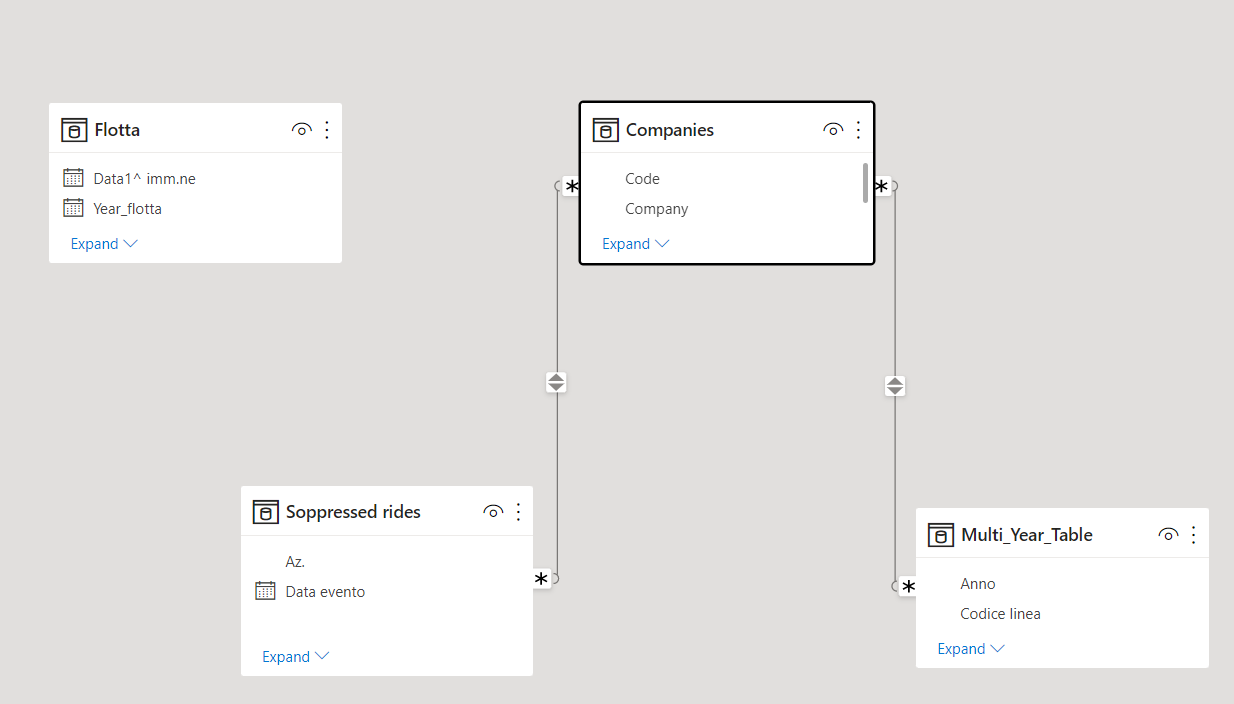
\includegraphics[width=0.9\textwidth]{Images/traditional_dashboard/ER_model.png}
    \caption{ER model of the Dashboard}
    \label{fig:ER}
\end{figure}
\section{Dashboard}

Starting from these tables, a dashboard is designed. It will be divided in subcategories that differ each other for the topic shown. In particular, the themes approached are:
\begin{itemize}
\item Suppressed rides
\item Emissions
\item Operative performances
\item KPIs correlation
\item Economics
\end{itemize}
\subsection{Suppressed rides}
In the following page has been presented the dashboard
\newpage
\begin{landscape}
\thispagestyle{empty}
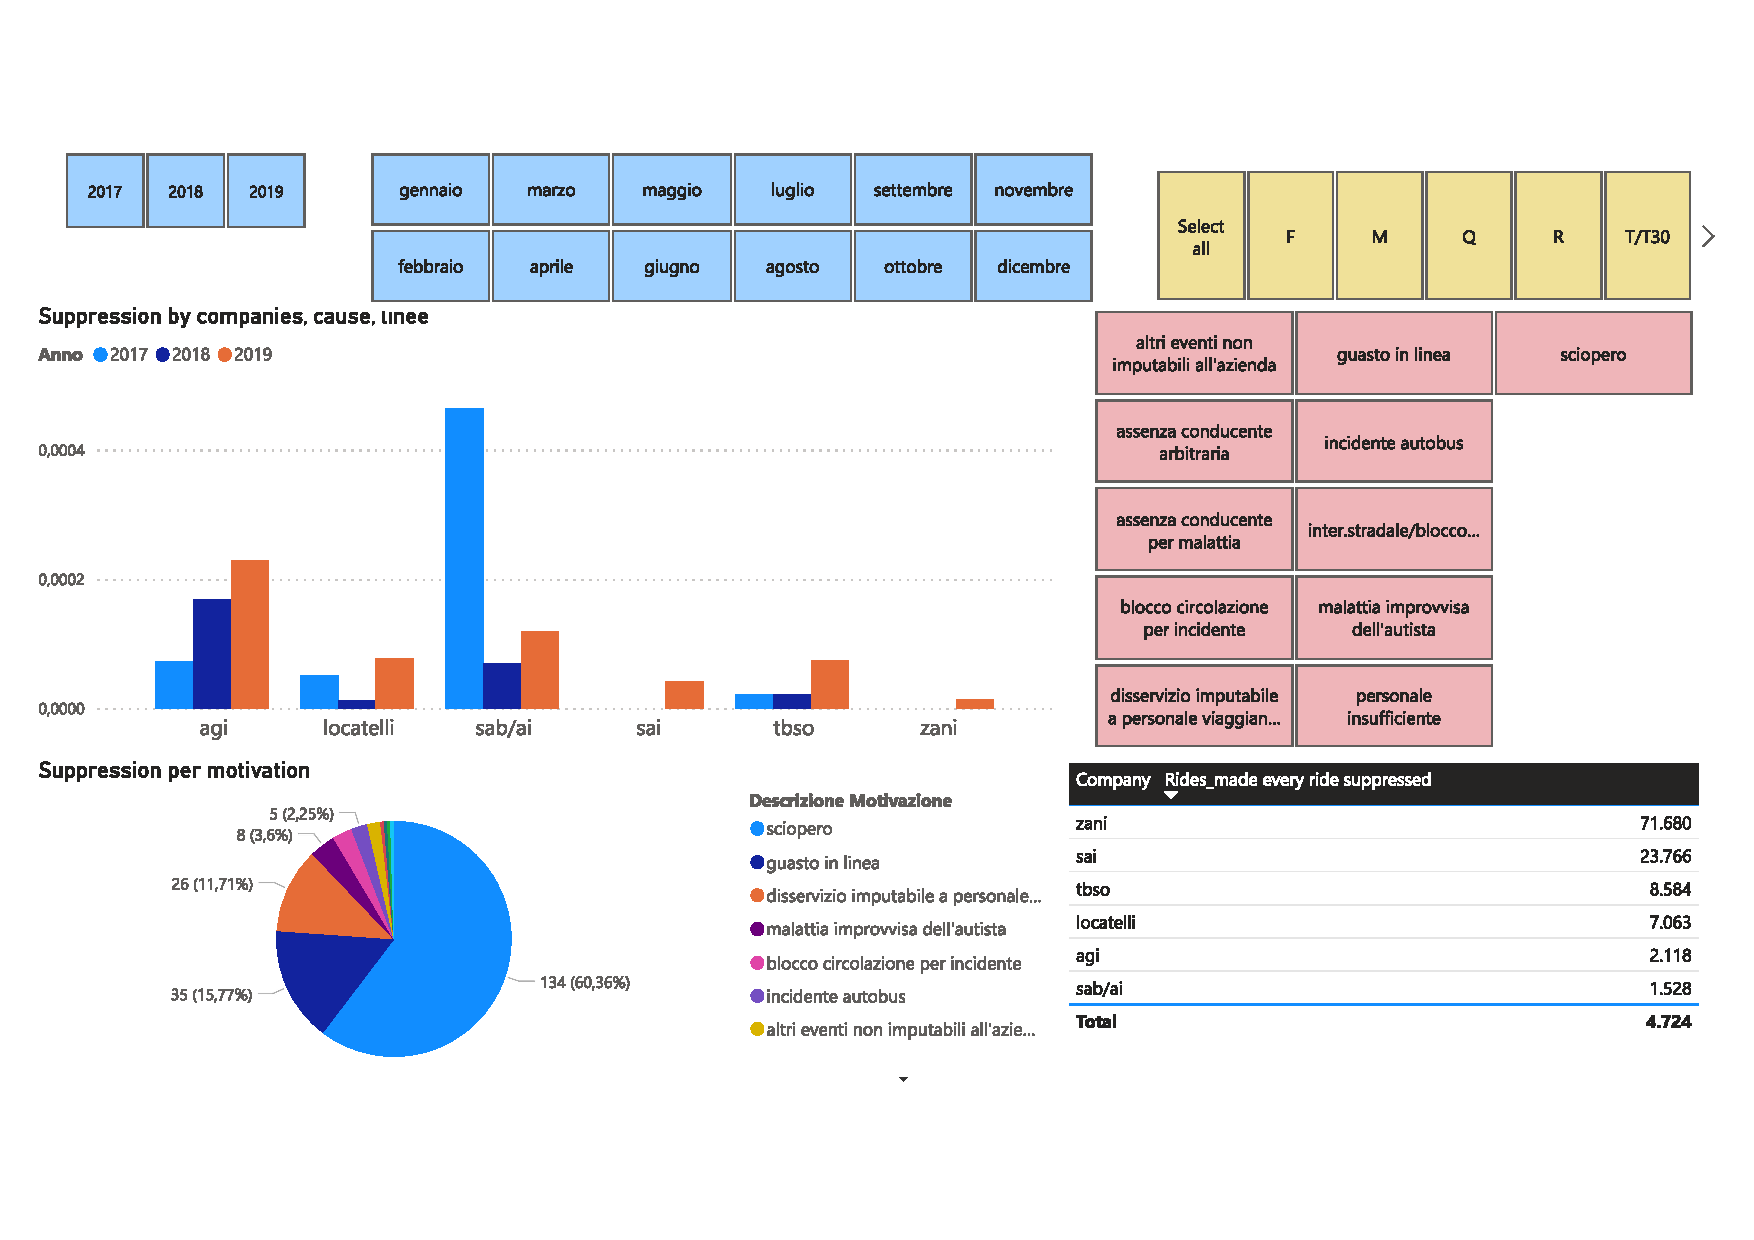
\includepdf[angle=90, pagecommand={\null\enlargethispage{2\baselineskip}\vfill\captionof{figure}{Suppressed}}]{dashboard/Suppression.pdf}
\end{landscape}
\newpage
As said before, data about suppressed rides are between 2017 and 2019. An area of this part of the page is dedicated to filters, thanks to which data can be visualized according to:
\begin{itemize}
\item  period of time with a level of detail equal to a month
\item line
\item reason for which the ride was suppressed
\end{itemize}
Obviously, these filters could be used at the same time in order to obtain very specific analysis.

The table on the bottom right shows the number of rides traveled per each ride suppressed for each company. So, a low number corresponds to a bad result for the company. This data is computed in a relative way in order to show if a company has bad performances according to its dimension. A ride suppressed for a small company is not comparable with few rides suppressed for a big one. 

The pie chart has the goal of showing how the different causes affects suppressed rides, while the histogram shows the total suppressed rides for each year divided by company. 

Considering the dashboard without applying any filter, some considerations can be already done. In 2017 Sab/ai had a huge issue with suppressed rides that reached a percentage level double than the second highest one, in the analyzed period. In 2017 and 2018 Sai and Zani had no problems and their suppressed rides are equal to zero. Finally, Agi had a ever increasing problem related to suppressed rides. 

Moreover, the main cause that brings to a suppressed ride is strike followed at a distance by failure happened during service and inconvenience due to drivers during service. 

Finally, companies with performances below Consortium average are Agi and Sab/ai with, respectively, a ride suppressed every 2,118 and 1,528 rides traveled. 

\newpage

\begin{landscape}
\thispagestyle{empty}
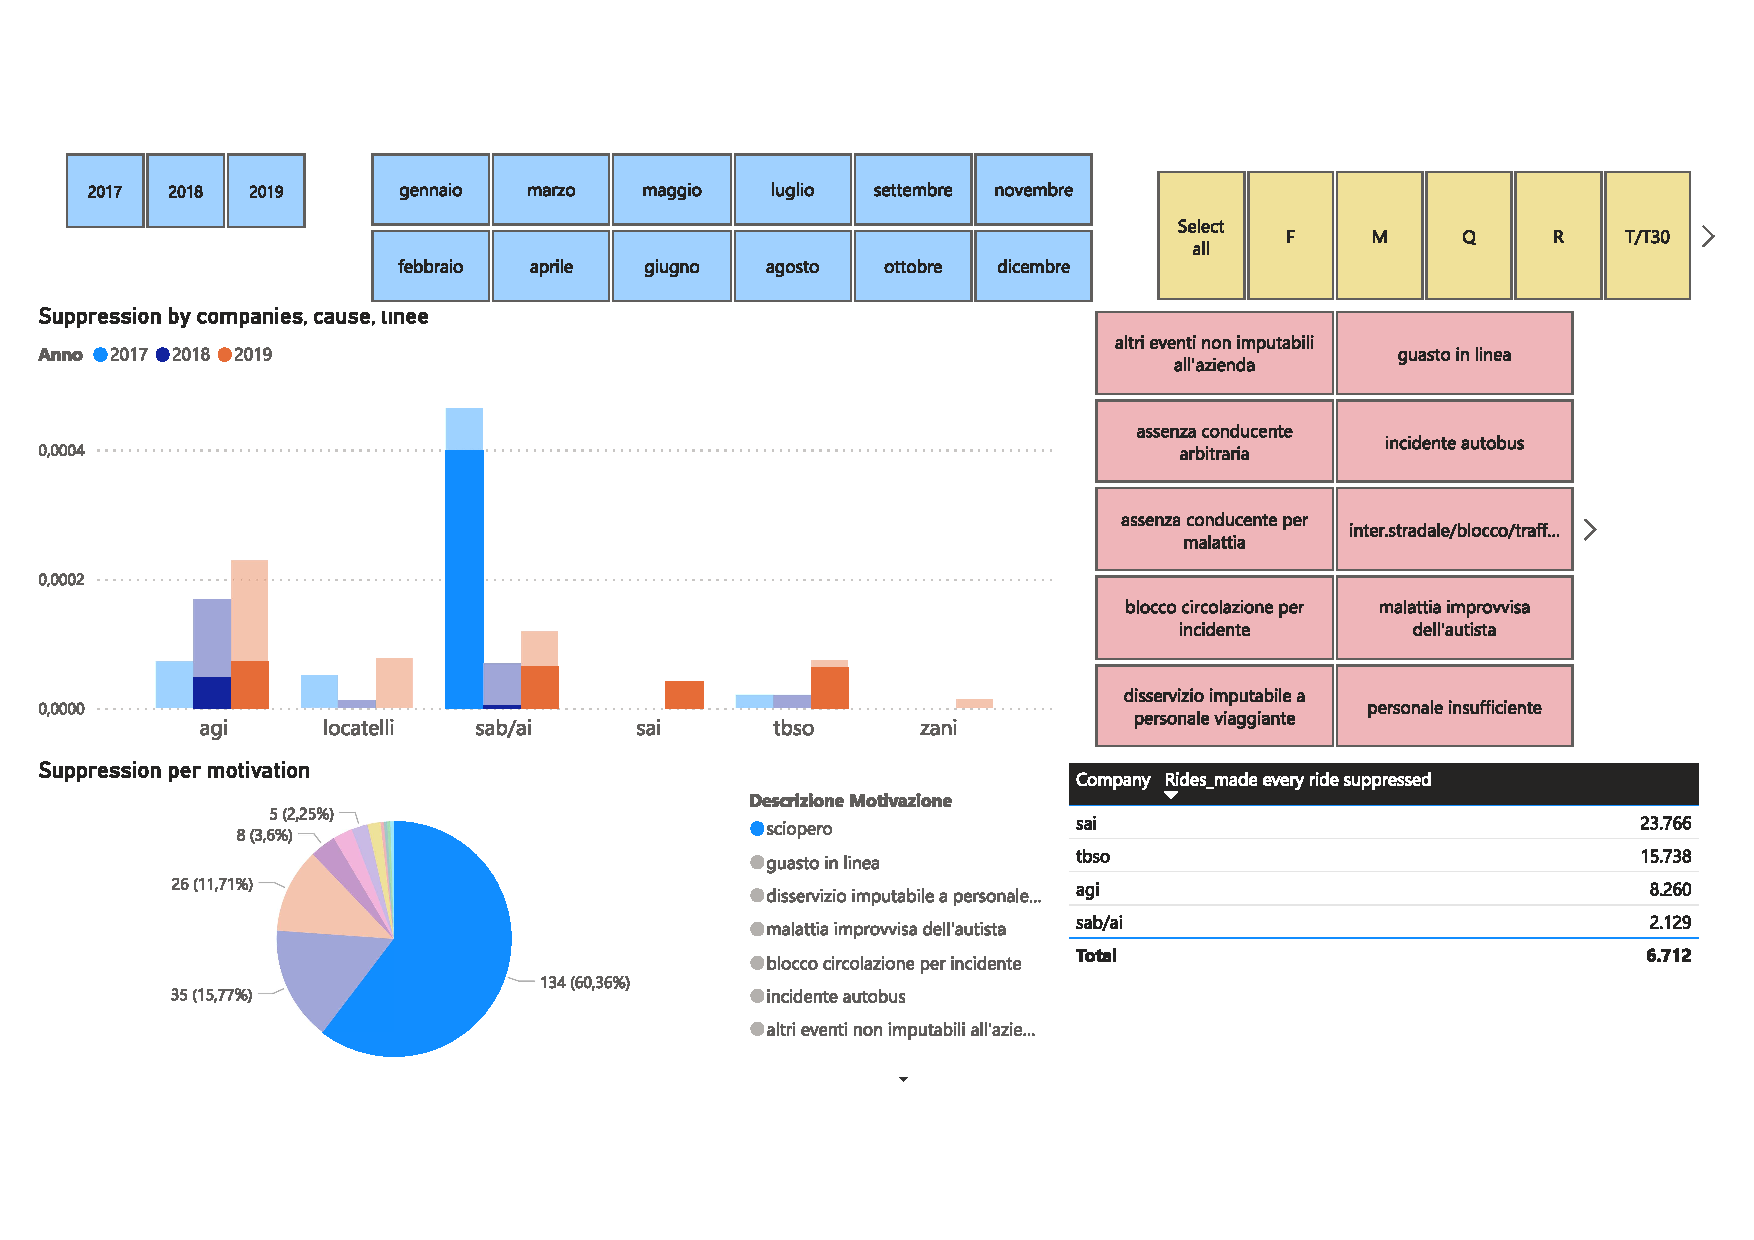
\includepdf[angle=90,  pagecommand={\null\enlargethispage{2\baselineskip}\vfill\captionof{figure}{Suppressed for strikes}\label{fig:strikes}}]{dashboard/Suppression_for_strikes.pdf}
\end{landscape}
\newpage

A focus on the strikes, shown in figure \ref{fig:strikes}, gives several information. Strikes are the reason of the abnormal problems tha Sab/ai had in 2017, moreover a strike in 2019 hit almost every company in an equal measure and, finally, Agi growing issues during this period are reflected also in strikes trend. 

Filtering data according to failure happened during service, a very interesting result is shown: half of the total failures happened during the three year in the Consortium happened during a ride performed by Agi even if Agi is one of the companies with less kilometers run per year. Moreover, this problem in absolute terms remains constant during the year and the negative trend of Agi is due to the increasing of other issues that in 2017 were almost absent.

\newpage
\begin{landscape}
\thispagestyle{empty}
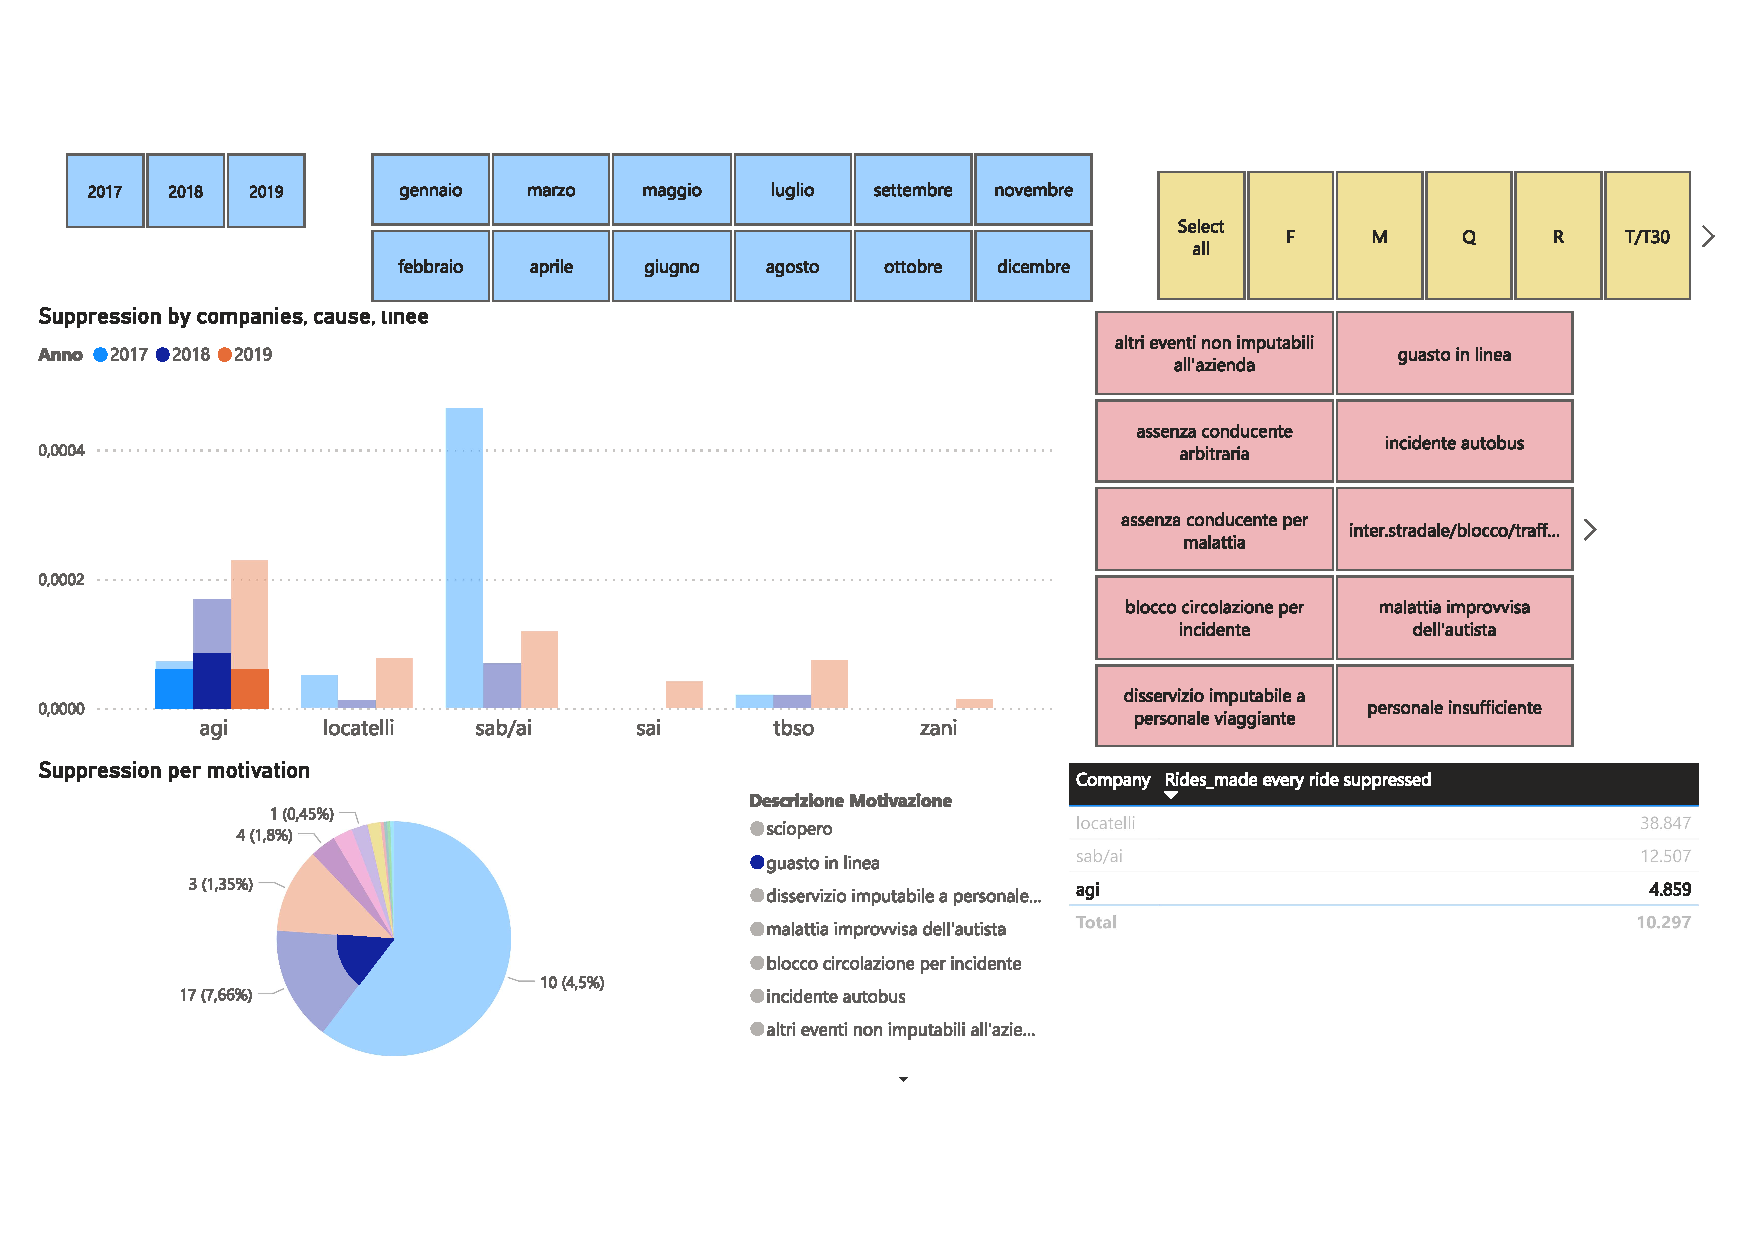
\includepdf[angle=90, pagecommand={\null\enlargethispage{2\baselineskip}\vfill\captionof{figure}{Focus on Agi and fault on the line}\label{fig:failline}}]{dashboard/Suppression_for_fail_on_the_line.pdf}
\end{landscape}
\newpage

\subsection{Fleet}

The second part of the dashboard regards an overview of the fleet based on the aspect that are underlined in the contract of service and that should be considered as constraint for a good fleet management, even if not all of them brings directly to a penalty from the Public Transport Authority. 
In particular, in the contract the PTA requires the following fleet criteria:
\begin{itemize}
\item $100\%$ buses must be air-conditioned
\item $91\%$ accessible for people with reduced mobility
\item  $100\%$ eco-diesel
\item at least $62\%$ Euro V, Euro VI, EEV or technologies with better emission performances.
\item  age restrictions:
    \begin{itemize}
        \item No restrictions if the age is lower of 18 years
        \item Travel limitation between 19 and 21 years, they can't be over $20\%$ of the total fleet
        \item Not allowed if they are over 22 years
    \end{itemize}
\end{itemize}
The figure \ref{fig:fleet}
shows the fleet situation in 2020, that is the most recent situation available. Data about 2018 and 2019 fleet are also available, so that comparison between these years can be done. Each aspect listed before is summed up in a pie chart that let a clear visualization of the situation.

Beginning from the good aspects, the entire fleet uses an eco-diesel fuel and almost every bus is equipped to allow the transport of people with reduced mobility. 
In Italy the average fleet age is about 12 years\cite{rossiPTM}, but in 2020 the Consortium results are even better with an average age of about 10 years. Despite this, 10 buses have an age that obliges them to suffer travel limitations and the $13\%$ in the immediate future will be in this situation. 
On the other side, as much as 8 buses are not equipped with air conditioning and, according to the contract of service, they should not travel. Finally, it is possible analyze the fleet according to their emission category. The requirements set by the contract ($62\%$) are widely satisfied, but the improvement margin is really high since the $30\%$ of the fleet has an high polluting engine. 


\newpage
\begin{landscape}
\thispagestyle{empty}
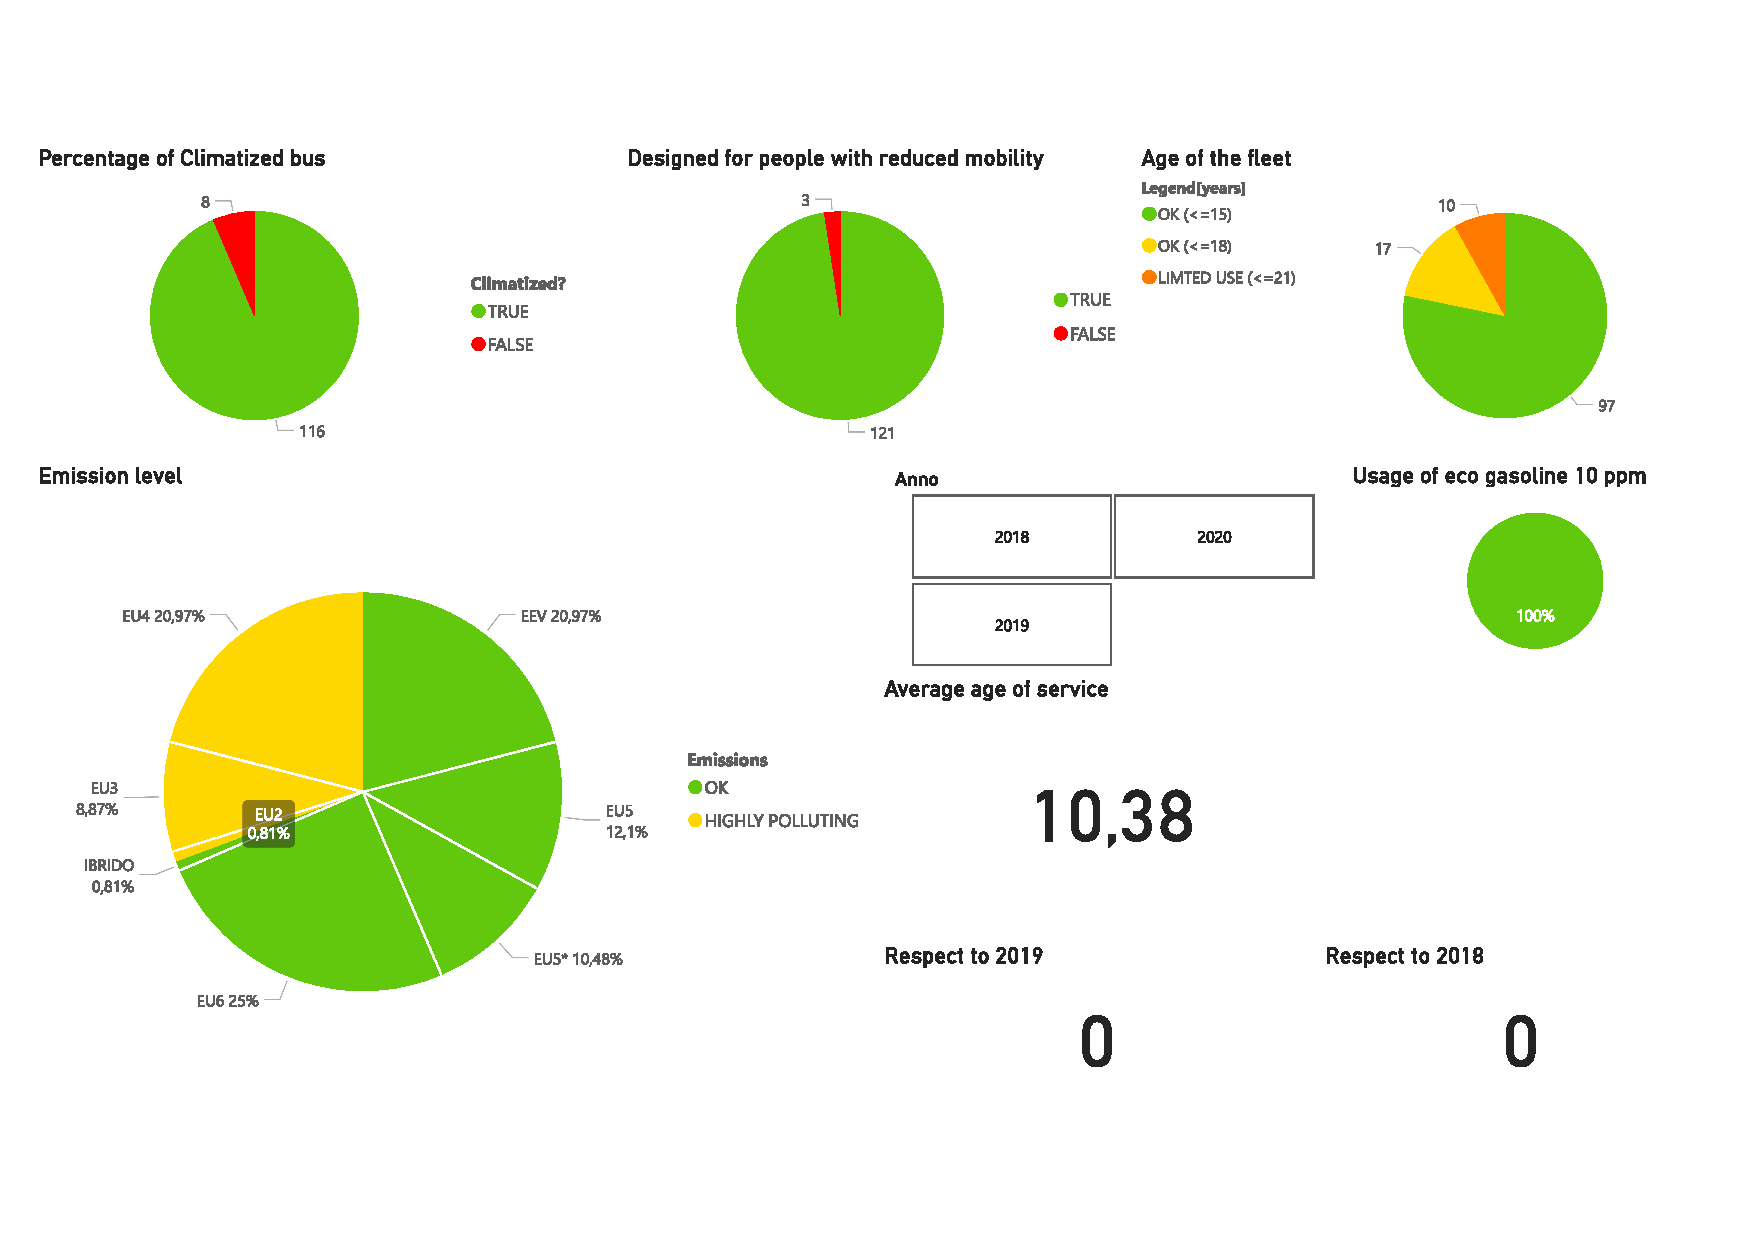
\includepdf[angle=90, pagecommand={\null\enlargethispage{2\baselineskip}\vfill\captionof{figure}{Fleet dashboard}\label{fig:fleet}}]{dashboard/emission.pdf}
\end{landscape}
\newpage

In the figure \ref{fig:fleetold}  a focus on the oldest part of the fleet in 2020, the one that has constraint on traveled kilometers. 
It can be seen that the majority of those buses are also the ones that are not air-conditioned, so, if they are replaced with new ones, two bad situations can be improved . Moreover, two of the three buses not equipped for people with reduced mobility belongs to this category. Unfortunately, if they are removed, an important percentage of not polluting buses would be lost. In fact, the $5\%$ of the fleet is composed of old buses with a swapped engine in order to respect contract limitations. Finally, the presence of buses with an age over 17 years is really increased respect to 2018, with a rise of over $200\%$.

\newpage
\begin{landscape}
\thispagestyle{empty}
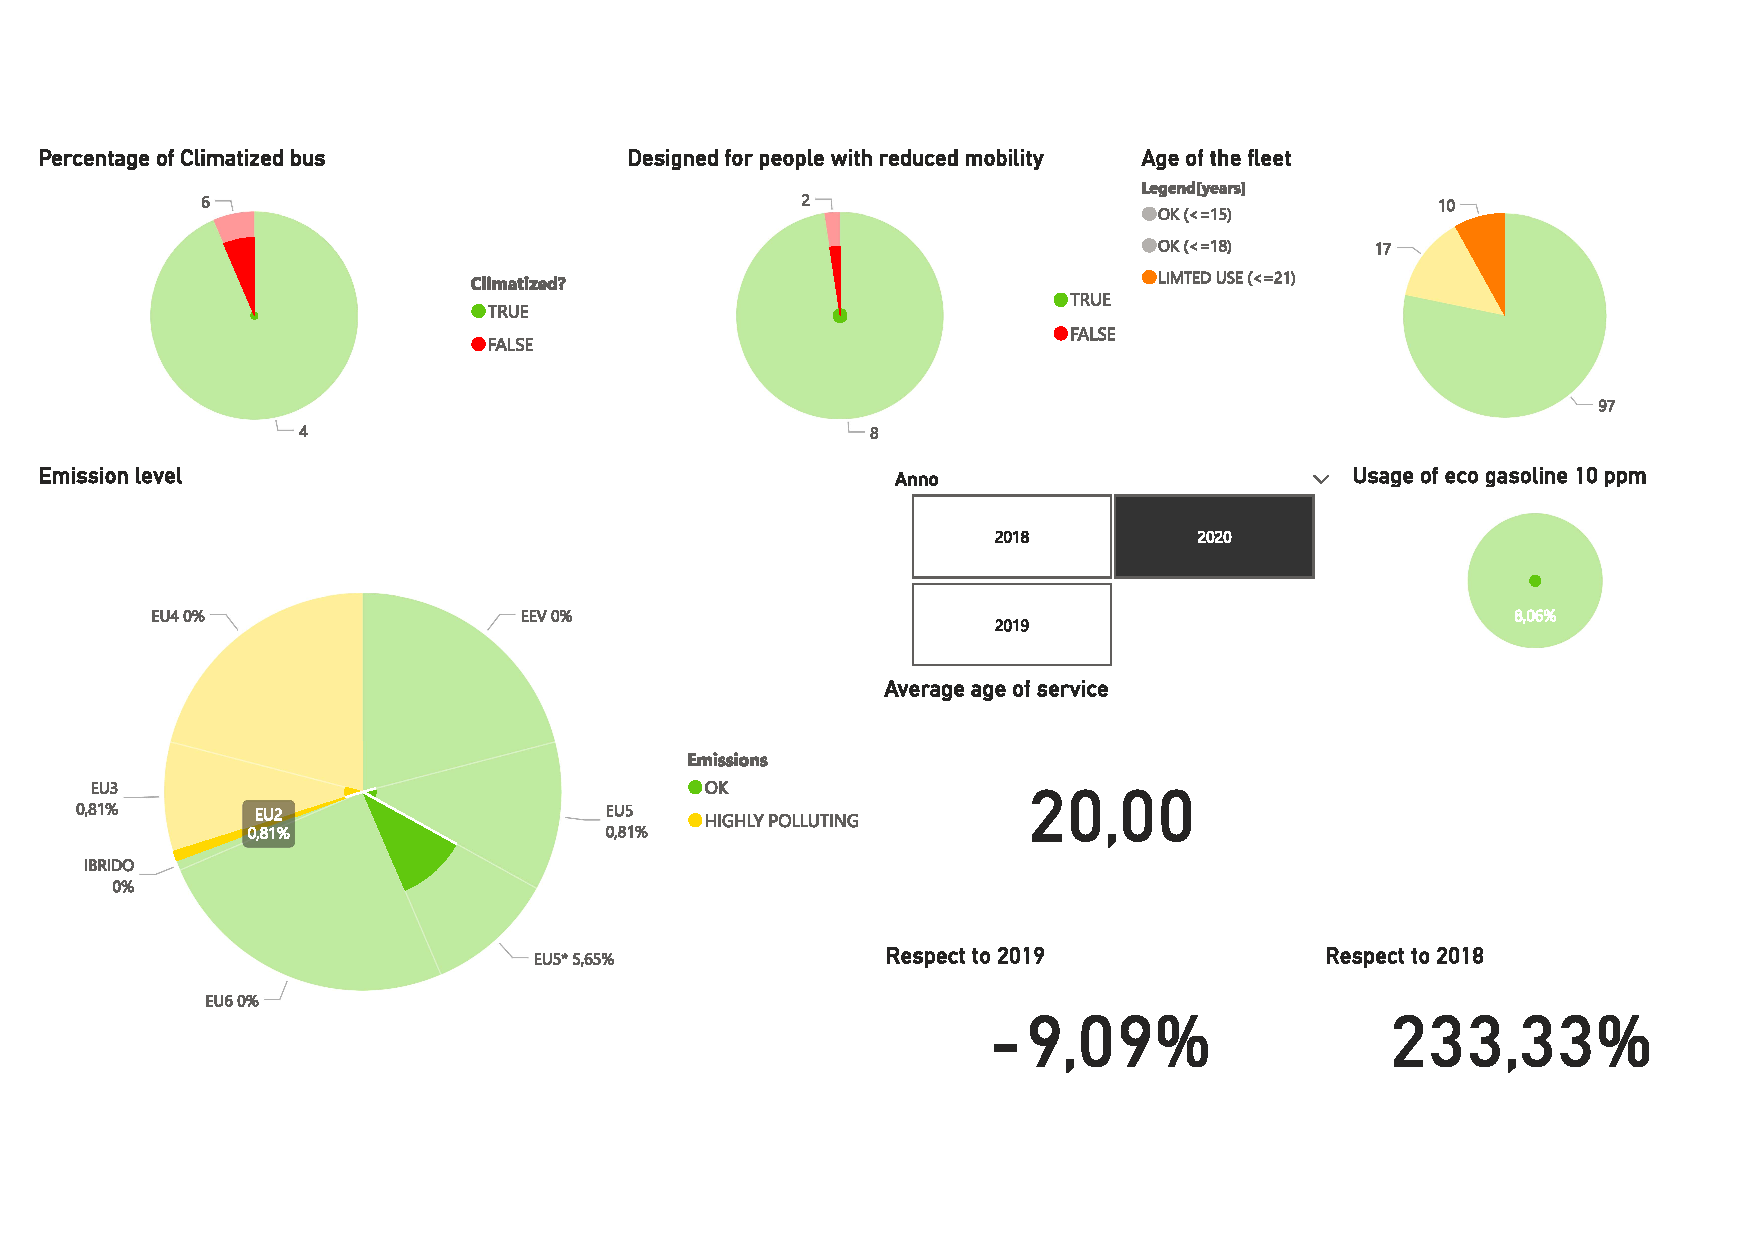
\includepdf[angle=90, pagecommand={\null\enlargethispage{2\baselineskip}\vfill\captionof{figure}{Focus on old fleet}\label{fig:fleetold}}]{dashboard/fleet_old_2020.pdf}
\end{landscape}
\newpage

